

    \begin{figure}
            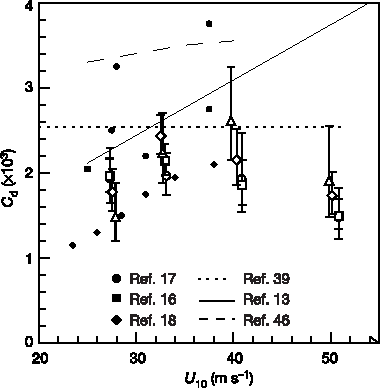
\includegraphics[width=1\linewidth]{images/example-images/cd.pdf}
                \caption{Fig. 3c from Powell 2003~\cite{powell2003reduced},
                 where they suggested that at high wind speeds $c_d$ decreases.}
    \end{figure}
\begin{figure}[htb!]
    \centering
    \includegraphics[width=1\linewidth]{../surge/plots/cd_finder.pdf}
    \caption{ Extracting $C_d$ from data.
    $ r_p = 0.9774 \pm 0.001,\;\; p<10^{-300}$\\
    $ m = 0.0383 \pm 0.0001 $ kg$^{0.5}$ m$^{-1.5}$\\
    $\implies  c_d = 0.001467 \pm 0.000008$ kg m$^{-3}$
    % error estimated from differences in output between test/training year,
    % measured regression error in either year much smaller than this.
    % The error is propogated using the \texttt{python3.uncertanties} package}
    There might be a theoretical limit~\cite{donelan2004limiting}.
    }
    %\label{fig:}
\end{figure}
